\chapter{Results}

\section{Simulated Data}

\subsection{Test Cases}

The test cases looked at were selected to determine the effects of the spacecraft inertia, the spacecrafts orbit and its geometry. In Total 18 total cases were simulated, each at multiple different time of the year and multiple random angular velocities.

The geometries used in this analysis were a rectangular prism, a cylinder, and a box-wing. The first two are convex geometries that have differing levels of symmetry, while the box-wing geometry is concave. The orbits examined are low, medium and geostationary Earth orbits. The final variable is the spacecrafts inertia. In the first case, the pricipal inertial axes are assumed to be aligned with the spacecraft body frame and equal. The effect of this is to make the spin axis constant for all time. In the second case, the principal inertial axes are all different and are not aligned with the body frame, causing the spin axis to change over time.

\begin{figure}\label{simulated_geometries}
	\begin{tabular}{cc}
		\includegraphics[width = 65mm]{Long_Rectangle_Image_Axes.png} &
		\includegraphics[width=65mm]{Cylinder_Axes} \\
		Rectangular Prism & Cylinder \\
		\multicolumn{2}{c}{\includegraphics[width=65mm]{Box_Wing_Axes}} \\
		\multicolumn{2}{c}{Box Wing}
	\end{tabular}
	\caption{Three Simulated Geometries.}
\end{figure}


\begin{figure}
	\begin{tabular}{cc}
		\includegraphics[width = 65mm]{leo_orbit} &
		\includegraphics[width=65mm]{meo_orbit} \\
		Low Earth Orbit & Medium Earth Orbit \\
		\multicolumn{2}{c}{\includegraphics[width=65mm]{geo_orbit}} \\
		\multicolumn{2}{c}{Geostationary Orbit}
	\end{tabular}
	\caption{Three Simulated Orbits.}
\end{figure}

\subsection{Simulation Methodology}

First, a LEO, MEO, and GEO orbit were selected. Passes were calculated by brute force sampling a spacecrafts location and checking for necessary conditions. These conditions were obviously that the spacecraft must be above the horizon of the observation site and that the spacecraft be illuminated. Passes lower than 20 degrees elevation were discarded. Additionally, in preliminary experiments it was noticed that the UKF often failed to converge to a solution when the solar phase angle (SPA) was greater than 90 degrees. Therefore passes with an SPA greater than 90 degrees were also discarded. Passes were also limited to only 5 minutes of data collection as MEO spacecraft passes can be hours long and geostationary passes are of course perpetual.

Once a pass was identified, the spacecraft was given three initial attitudes and angular velocities between 0.1 and 0.3 radians per second. These were then propagated and used to calculate three different light curves per pass. Before entering the Kalman Filter, Gaussian noise was added to the light curve whose distribution was similar to that of the real data collected.

The inertia matrix used for the spacecraft in the tumbling cases was as follows:
\begin{equation}
\begin{bmatrix}
1 & .01 & .01 \\ .01 & 2 & .01 \\ .01 & .01 &3
\end{bmatrix}
\end{equation}

This matrix follows the assumptions used in the derivation of the UKF formulation. These being that the offdiagonal elements are small and therefore negligible. 
\subsection{Simulation Results}

\subsubsection{Existence of Multiple Solutions}
The simulation results reveal that the problem of uniquely identifying an attitude profile from a light curve is an indeterminate problem. The data shows that for any light curve, there are multiple combinations of attitude profiles and angular velocities that can produce it. Many of these solutions are a result of the symmetry of the spacecraft. For example, a rectangular prism rotated by 180 degrees about any axis will appear indistinguishable from its original orientation assuming that each face has identical reflectance properties.

Another source of indeterminacy comes from the truth that it is impossible to distinguish between an object rotating about an axis clockwise and counterclockwise. Therefore, in this thesis, only the axis of rotation is examined. What this means is that, during analysis, the estimated angular velocity was multiplied by 1 or -1 to minimize the dot product between the true angular velocity and estimated angular velocity. This simply serves to make valid results more apparent.


\subsubsection{Convergence Criteria}
 
Convergence was determined by examining the magnitude of the update to the angular velocity. If it was seen that the angular velocity was changed less than $1\times 10^{-4}$ radians/second in each axis the UKF was said to converge.

For the cases where angular velocity was held constant, this resulted in very satisfactory results. However, in the cases where the angular velocity was not constant, the UKF would meet the convergence criteria without producing a realistic solution. The successful runs of the UKF for these cases were then hand selected using the criteria that a valid solution for angular velocity should appear sinusoidal and not change dramatically in amplitude or period.

\subsubsection{Methodology}

One challenge to analyzing this data occurs because of the multiple solutions which appear. In these cases, there is no ground truth to compare performance against. This would not be an issue if these alternate solutions were the minority of solutions found as they could simply be discarded. However, these alternative solutions are by far the majority.

In order to yield meaningful results without reducing the sample size to only a handful of cases, the following methodology was applied to the data. If any component of the angular velocity fell within 10\% of the ground truth, it was considered to be converging towards it and its error would be added to the statistics. This runs the risk of sample bias as this guarantees that the performance will be better than 10\% for every axis. However, the results show that the actual performance was significantly better than 10\% which implies that the majority of the data was correctly accounted for.

Angular velocities were analyzed in two frames: The body frame and the observation frame. The body frame is the reference frame fixed to the spacecraft body. In this frame, direct comparisons can be made to the ground truth and deductions can be made about performance wiith respect to the spacecraft geometry. The inertial interpretation of the angular velocity in body frame is dependant on the spacecraft attitude. As it can be shown that multiple attitudes can result in the same light curve, the body frame serves as a poor frame to analyze angular velocities which may appear wildly different in body frame but which closely mirror the ground truth when the spacecraft attitude is accounted for. The best frame to analyze this is the Observation frame.

%include plot of the OBSERVATION frame

The observation frame is defined to have its origin at the center of the spacecraft, its X axis along the observation vector, the Z axis being the cross of the sun and observation vector, and the Y axis completing the frame. This frame enabled comparisons between the estimated and true angular velocities in a frame which is irrespective of the spacecrafts attitude. Additionally, this frame allows for the error analysis with respect to the geometry of the situation. E.g, the direction of observation and illumination with respect to the spacecraft.

\subsubsection{Hypothesis}

This thesis hypothesizes that a second, predicable set of solutions exists which can recreate a given lightcurve. This second set of solutions is characterized by an angular velocity vector whose magnitude and direction are directly mirrored across the plane of the observation.

It can be noticed in the formulation of the measurement model that measured light intensity is a function of the relative directions of the facet normals, observation, and velocity vectors. Therefore, if one imagines a mirror floating beneath the spacecraft in the observation plane (The XY plane of the observation frame), it can be visualized that it would result in an identical lightcurve.

This is only possible when the observational plane remains relatively constant however. As the observational plane changes, so must the mirrored angular velocity. As the UKF used in this thesis assumes that the angular velocity is either constant or changes according to Eulers equations of rigid body motion. This unmodeled motion usually excludes the mirrored solution as valid.


\subsubsection{Case: Fixed Axis of Rotation}

\begin{table}[ht]
	\begin{center}
		\begin{tabular}{| c | c | c | c | c |}
			\hline Geometry & LEO & MEO & GEO & Total Trials\\ 
			\hline Cylinder & 52.77\% & 48.88\% & 69.44\% & 117 \\
			\hline Rectangular Prism & 19.44\% & 57.77\% & 63.88\% & 117\\
			\hline Box-Wing & 0.00\% & 50.00\% & 86.95\% & 80\\
			\hline
		\end{tabular}
	\end{center}
	\caption{Percentages of Trials with Converged Solutions: Fixed Axis Case}
\end{table}

\begin{figure}[ht]
	\begin{center}
		\includegraphics[width = 85mm]{Body_Errorbars}
		\caption{Body Rate Error}
	\end{center}
\end{figure}

The first result is that the UKF performs significantly better in the Geostationary cases. Excepting the cylinder case, where the LEO and MEO had similar success rates, it seems that LEO is the most challenging for the UKF.

This is likely due to the fact that in both MEO and LEO, the amplitude of the light curve can vary dramatically across the pass as the objects distance from the observer changes. This means that small errors in the state estimate correspond to different magnitude errors depending on when they occur during the pass. This is to say that the model uncertainty changes throughout the pass while the UKF assumes it is constant. The reason MEO performs better than LEO is because a MEO object near apogee has a very constant amplitude. In GEO, the spacecraft effectively do not change their distance from the observer and so their model uncertainty remains extremely constant.

\begin{table}[ht]
	\begin{center}
		\begin{tabular}{| c | c | c | c |}
			\hline Geometry & \multicolumn{3}{c}{Angular Velocity  Error - Body Frame}\\ 
			\hline Cylinder & $4.26E-3 \pm 2.08E-3$ &
							 $7.12E-3 \pm 3.32E-3$ &
							 $9.04E-4 \pm 3.05E-4$ \\
			\hline Rectangular & $2.64E-3 \pm 7.94E-4$ &
								 $2.64E-3 \pm 8.64E-4$ &
								 $1.84E-3 \pm 6.21E-4$ \\
			\hline Box-Wing & $1.52E-3 \pm 3.39E-3$ &
							  $5.25E-3 \pm 2.55E-3$ &
							  $5.70E-3 \pm 1.14E-3$ \\
			\hline
		\end{tabular}
	\end{center}
	\caption{Error Bounds for Various Geometries in Body Frame}
\end{table}

It can be see that in the body frame, the cylinder geometry had significantly less error about its Z-axis which corresponds to its length. In figure \ref{simulated_geometries} it can be seen that the cylinder model is modeled as a set of flat facets. It is likely that as the number of facets increases that the error along the Z axis also increases. This is because as the cylinder rotates each facet bightens and then dims, creating a low bumps in the intensity signal that would not be caused by a true cylinder. These "bumps" very likely make it easier for the UKF to converge on the Z axis angular velocity.

In general the box wing geometry has large error compared two the other two. This is in part due to the fact that this geometry was the smallest geometry and so the modeled noise affected the signal proportionately more. It can be seen that the X-axis of the geometry had significantly higher error than the other axes. This is likely do with the fact that this axis was the one along which the wings were placed. Error about the other axes would affect the location of the wings and therefore the overall brightness much more than error along the X-axis.


\begin{table}[ht]
	\begin{center}
		\begin{tabular}{| c | c | c | c |}
			\hline Geometry & \multicolumn{3}{c}{Angular Velocity Error - Observation Frame} \\ 
			\hline Cylinder & 
			$3.03E-3\pm 1.23E-3$ &
			$1.38E-3 \pm 7.21E-4$ &
			$5.53E-4 \pm 7.97E-5$ \\
			\hline Rectangular &
			$4.96E-3 \pm 1.66E-3$ &
			$3.80E-3 \pm 1.45E-4$ &
			$1.42E-3 \pm 4.35E-4$ \\
			\hline Box-Wing &
			$2.50E-3 \pm 8.57E-4$ &
			$2.11E-3 \pm 2.19E-4$ &
			$5.71E-3 \pm 2.37E-3$ \\
			\hline
		\end{tabular}
	\end{center}
	\caption{Error Bounds for Various Geometries in Observation Frame}
\end{table}

\begin{figure}[ht]
	\begin{center}
		\includegraphics[width = 85mm]{OBS_Errorbars}
		\caption{Observation Frame Rate Error}
	\end{center}
\end{figure}


Looking that the error in the Observation Frame, both the cylinder and rectangular prism geometries showed significantly reduced error along the Z axis. By looking at equations \ref{Phong_Specular} and \ref{Phong_Diffuse}, it can be seen that the amount of power reflected is a function of the sun and observation vectors which lie along the XY plane of the Observation frame. It can be intuited that any error in the component of angular velocity normal to both the observation and sun vector would would have the largest effect on the predicted measurement. Therefore the angular velocity along the Z component of the Observation Frame is the most likely to be corrected by the UKF.

\begin{figure}[ht]
	\begin{tabular}{cc}
		\includegraphics[width = 50mm]{figures/Rectangle_Leo/BODY} &
		\includegraphics[width=50mm]{figures/Rectangle_Leo/CURVE} \\
		Angular Velocity in Body Frame & Light Curve Comparison \\
		\includegraphics[width = 50mm]{figures/Rectangle_Leo/OBS} &
		\includegraphics[width = 50mm]{figures/Rectangle_Leo/MRP} \\
		Angular Velocity in Observation Frame & Modified Rodrigues Parameter Comparison
	\end{tabular}
	\caption{Converged Solution of a Rectangular Prism in LEO spinning About a Fixed Axis.}
\end{figure}


\begin{figure}[!ht]
	\begin{tabular}{cc}
		\includegraphics[width = 50mm]{figures/Cylinder_Leo/BODY} &
		\includegraphics[width=50mm]{figures/Cylinder_Leo/CURVE} \\
		Angular Velocity in Body Frame & Light Curve Comparison \\
		\includegraphics[width = 50mm]{figures/Cylinder_Leo/OBS} &
		\includegraphics[width = 50mm]{figures/Cylinder_Leo/MRP} \\
		Angular Velocity in Observation Frame & Modified Rodrigues Parameter Comparison
	\end{tabular}
	\caption{Converged Solution of a Cylinder in LEO Spinning About a Fixed Axis.}
\end{figure}

\begin{figure}![ht]
	\begin{tabular}{cc}
		\includegraphics[width = 50mm]{figures/BW_Geo/BODY} &
		\includegraphics[width=50mm]{figures/BW_Geo/CURVE} \\
		Angular Velocity in Body Frame & Light Curve Comparison \\
		\includegraphics[width = 50mm]{figures/BW_Geo/OBS} &
		\includegraphics[width = 50mm]{figures/BW_Geo/MRP} \\
		Angular Velocity in Observation Frame & Modified Rodrigues Parameter Comparison
	\end{tabular}
	\caption{Converged Solution of a Box-Wing in GEO Spinning About a Fixed Axis}
\end{figure}

\subsubsection{Case: Tumbling Spacecraft}

\begin{table}[!ht]
	\begin{center}
		\begin{tabular}{| c | c | c | c | c |}
			\hline Geometry & LEO & MEO & GEO & Total Trials\\ 
			\hline Cylinder & 22.00\% & 25.00\% & 25.00\% & 108 \\
			\hline Rectangular Prism & 2.77\% & 2.77\% & 16.66\% & 108\\
			\hline Box-Wing & 0.00\% & *0.00\% & *41.37\% & 101\\
			\hline \multicolumn{5}{c}{* Spacecraft truth model had no off-diagonal elements.} \\
			\hline
			
		\end{tabular}
	\end{center}
	\caption{Percentages of Trials with Converged Solutions: Tumbling Case}
\end{table}

The success rates for the tumbling cases were far lower than in the fixed axis case. This is to be expected however as the number of parameters to estimate and the complexity of the models are significantly greater. Again though, we see the pattern in which performance increases with orbital altitude.

Another trend which has continued into the tumbling case is that there are once again multiple solutions which result in the same predicted measurement. In this new data we see solutions converging with variations in period and amplitude in addition to magnitude and direction. These extra degrees of freedom could potentially be why the UKF struggles to settle on a single solution.

In regards to the Inertia estimation, results varied wildly. It is known that in the absence of disturbances only the relative magnitude of the inertia values matter. The top left element was forced to be 1, and the other two diagonal elements were expected to converge to the true values. What was seen in the data however was that the inertia values often converged to values which differed from the truth, but preserved the same ratios between inertial axes.

\begin{figure}![ht]
	\begin{tabular}{cc}
		\includegraphics[width = 50mm]{figures/Cylinder_Meo_Tumbling/BODY} &
		\includegraphics[width=50mm]{figures/Cylinder_Meo_Tumbling/CURVE} \\
		Angular Velocity in Body Frame & Light Curve Comparison \\
		\multicolumn{2}{c}{\includegraphics[width=50mm]{figures/Cylinder_Meo_Tumbling/INERTIA}}\\
		\multicolumn{2}{c}{Estimated Inertia Values}
	\end{tabular}
	\caption{Converged Solution of a Box-Wing in GEO Spinning About a Fixed Axis}
\end{figure}

\begin{figure}![ht]
	\begin{tabular}{cc}
		\includegraphics[width = 50mm]{figures/Rect_Meo_Tumbling/BODY} &
		\includegraphics[width=50mm]{figures/Rect_Meo_Tumbling/CURVE} \\
		Angular Velocity in Body Frame & Light Curve Comparison \\
		\multicolumn{2}{c}{\includegraphics[width=50mm]{figures/Rect_Meo_Tumbling/INERTIA}}\\
		\multicolumn{2}{c}{Estimated Inertia Values}
	\end{tabular}
	\caption{Converged Solution of a Box-Wing in GEO Spinning About a Fixed Axis}
\end{figure}


\begin{figure}![ht]
	\begin{tabular}{cc}
		\includegraphics[width = 50mm]{figures/BW_Geo_Tumbling/BODY} &
		\includegraphics[width=50mm]{figures/BW_Geo_Tumbling/CURVE} \\
		Angular Velocity in Body Frame & Light Curve Comparison \\
		\multicolumn{2}{c}{\includegraphics[width=50mm]{figures/BW_Geo_Tumbling/INERTIA}}\\
		\multicolumn{2}{c}{Estimated Inertia Values}
	\end{tabular}
	\caption{Converged Solution of a Box-Wing in GEO Spinning About a Fixed Axis}
\end{figure}


\subsubsection{Hypothesis Results}

By examining the angular velocities in the observation frame, it was observed that 6 of the 117 trials converged to a solution which was mirrored across the observational plane. This was apparent because, in the observation frame, the angular velocity converged to the correct axis and magnitude with the exception that the Z component was the negative of what the truth.

\begin{figure}[ht]
	\begin{tabular}{cc}
		\includegraphics[width = 65mm]{figures/flips/R_OBS} &
		\includegraphics[width=65mm]{figures/flips/R_CURVE} \\
		Angular Velocity in the Observation Frame & Light Curve Comparison
	\end{tabular}
	\caption{Example of a solution which is flipped across the observation plane.}
\end{figure}

\begin{figure}[ht]
	\begin{center}
		\includegraphics[width=140mm]{figures/flips/R_FRAMES}
	\end{center}
	\caption{Consecutive Images from the observers perspective of truth [TOP] and estimate [BOTTOM] showing a mirror image solution.}
\end{figure}

\section{Real Data}

\subsection{SERT-2}

The Space Electric Rocket Test II (SERT-2) is a modified Aegena rocket body whose mission was to test two ion propulsion systems on board. \cite{sert2} In order to power these propulsion systems, two deployable solar panels were added to the Aegena rocket body whose dimensions were 1.5x6 meters. The dimensions of the Aegena module were also 1.53x6 meters.

SERT-2 was launched on February 3rd, 1970 and was finally decommissioned in 1991. Due to the age of the spacecraft and considering that there is potentially fuel remaining within the Aegena tank, this spacecraft can be assumed to be spinning about its major axis. This obviously simplifies the UKF model and allows this thesis to implement the simpler version.

The geometry of SERT-2 is essentially a cylinder with two rectangular panels radiating from one end. This model is non-convex which means that it can take advantage of ray tracing algorithm described in this thesis. 

\begin{figure}[ht]
	\begin{tabular}{cc}
	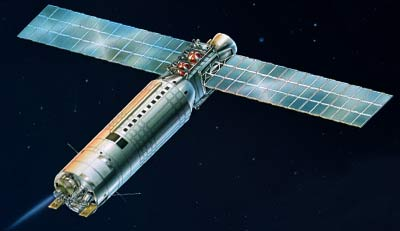
\includegraphics[width = 80mm]{figures/sert-2} & \includegraphics[width = 60mm]{figures/SERT2_Axes} \\
	SERT-2, Source: NASA & SERT-2 Reflectance Model 
	
	\end{tabular}
	\caption{SERT-2 vs Reflectance Model}
\end{figure}

\begin{figure}![ht]
	\begin{tabular}{cc}
		\includegraphics[width = 50mm]{figures/Sert_Success/BODY} &
		\includegraphics[width=50mm]{figures/Sert_Success/CURVE} \\
		Angular Velocity in Body Frame & Light Curve Comparison \\
		\includegraphics[width = 50mm]{figures/Sert_Success/ECI} &
		\includegraphics[width = 50mm]{figures/Sert_Success/MRP} \\
		Angular Velocity in ECI Frame & Modified Rodrigues Parameter Estimates
	\end{tabular}
	\caption{Convergence of a solution using real data of SERT-2.}
\end{figure}

% Table generated by Excel2LaTeX from sheet 'datatable'
\begin{table}[htbp]
	\centering
	
	\begin{tabular}{|l|r|r|r|r|r|r|}
		\hline & \multicolumn{1}{l}{X Body} & \multicolumn{1}{l}{Y Body} & \multicolumn{1}{l}{Z Body} & \multicolumn{1}{l}{X ECI} & \multicolumn{1}{l}{Y ECI} & \multicolumn{1}{l}{Z ECI} \\
		\hline 2018-06-02 & -0.03838 & 0.099123 & 0.276464 & -0.03607 & -0.20629 & -0.20946 \\
		\hline 2018-06-15 & 0.094913 & 0.307434 & -0.29946 & 0.4386 & -0.0136 & 0.025415 \\
		\hline 2018-06-23 & -0.0934 & -0.0615 & 0.547375 & 0.448295 & -0.31579 & -0.10693 \\
		\hline 2018-06-27 & 0.004656 & -0.00586 & -0.58329 & 0.29951 & -0.38325 & 0.322009 \\
		\hline 2018-07-02 & 0.012748 & 0.02757 & -0.68151 & -0.08979 & -0.67597 & -0.01929 \\
		\hline 2018-07-07 & 0.107008 & 0.096465 & 0.264944 & 0.206755 & -0.21221 & -0.05632 \\
		\hline 2018-07-16 & -0.00967 & -0.75654 & -0.00129 & -0.53145 & 0.385914 & -0.37562 \\
		\hline 2018-08-10 & -0.06039 & 0.011915 & 0.613305 & -0.33712 & 0.489952 & 0.161957 \\
		\hline 
	\end{tabular}%
	\caption{Final Angular Velocity Vector of SERT-2 According to UKF Estimates.}
\end{table}%



\subsection{Ajisai (EGS)}

Ajisai was a mission launched on August 13th, 1986 and was primarily intended as a dummy payload for the H-I launch vehicle. \cite{ajisai_jaxa} Ajisai is essentially a sphere covered with 1,436 corner cube reflectors and 318 mirrors. \cite{ajisai} Its secondary mission (after being mass) was to determine the exact position of the more isolated Japanese islands. \cite{ajisai_jaxa}

Because this spacecraft is so old and because it is a sphere. It is highly likely that it is spinning about its major axis and the simpler UKF formulation can be applied once more.

\begin{figure}
	\begin{tabular}{cc}
	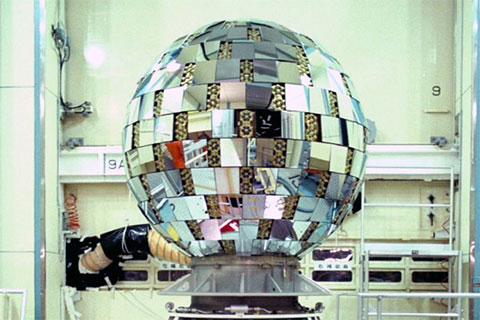
\includegraphics[width = 90mm]{figures/ajisai.jpg} & \includegraphics[width = 60mm]{figures/AJISAI_Axes} \\
	AJISAI, Source: JAXA & AJISAI Reflectance Model
	\end{tabular}
	\caption{AJISAI vs Reflectance Model}
\end{figure}



The geometry of the spacecraft is simply a large set of reflective panels. Being mirrors, these panels will have very high specular reflectance and almost no diffuse reflectance. The corner cube reflectors designed to reflect light back to its source. For this thesis, that source is the sun, and so the corner cube reflectors can be assumed to contribute nothing to the lightcurve. Thankfully, the positions of each corner cube reflector were documented, and the panel locations can be inferred from them.

\begin{figure}[ht]
	\centering
	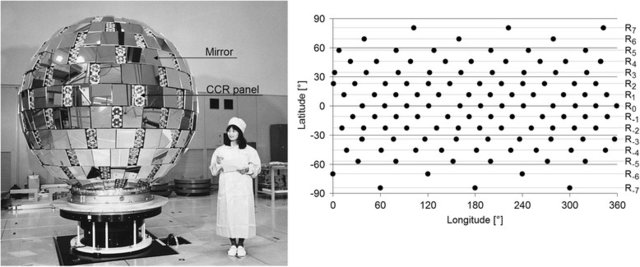
\includegraphics[width = 150mm]{figures/ajisai_panels.jpg}
	\caption{Ajisai with Engineer [Left]. Corner Cube Reflector Locations [Right] \cite{ajisai}}
\end{figure}

\begin{figure}![ht]
	\begin{tabular}{cc}
		\includegraphics[width = 50mm]{figures/Ajisai_Fail/BODY} &
		\includegraphics[width=50mm]{figures/Ajisai_Fail/CURVE} \\
		Angular Velocity in Body Frame & Light Curve Comparison \\
		\includegraphics[width = 50mm]{figures/Ajisai_Fail/ECI} &
		\includegraphics[width = 50mm]{figures/Ajisai_Fail/MRP} \\
		Angular Velocity in ECI Frame & Modified Rodrigues Parameter Estimates
	\end{tabular}
	\caption{Measurement model mismatch with real data from AJISAI.}
\end{figure}

\subsection{Ariane-40 R/B}

\begin{figure}[ht]
 \includegraphics[width = 60mm]{figures/ARIANE_Axes}
\caption{SERT-2 vs Reflectance Model}
\end{figure}

\begin{figure}![ht]
	\begin{tabular}{cc}
		\includegraphics[width = 50mm]{figures/Ariane_Success/BODY} &
		\includegraphics[width=50mm]{figures/Ariane_Success/CURVE} \\
		Angular Velocity in Body Frame & Light Curve Comparison \\
		\includegraphics[width = 50mm]{figures/Ariane_Success/ECI} &
		\includegraphics[width = 50mm]{figures/Ariane_Success/MRP} \\
		Angular Velocity in ECI Frame & Modified Rodrigues Parameter Estimates
	\end{tabular}
	\caption{Convergence of a solution using real data of Ariane-40 R/B.}
\end{figure}

% Table generated by Excel2LaTeX from sheet 'datatable'
\begin{table}[htbp]
	\centering
	
	\begin{tabular}{lrrrrrr}
		\hline & \multicolumn{1}{l}{X Body} & \multicolumn{1}{l}{Y Body} & \multicolumn{1}{l}{Z Body} & \multicolumn{1}{l}{X ECI} & \multicolumn{1}{l}{Y ECI} & \multicolumn{1}{l}{Z ECI} \\
		\hline 2018-09-23 & -0.00019 & -0.0013 & 0.951019 & 0.089868 & -0.87416 & 0.363605 \\
		\hline 2018-10-09 & -0.00721 & -0.0024 & 0.086334 & 0.083592 & -0.0225 & 0.004204 \\
		\hline 2018-10-20 & 0.001436 & 0.017491 & 0.003996 & -0.01783 & -0.00064 & 0.002395 \\
		\hline 2018-10-23 & -0.00812 & -0.01534 & -0.26552 & -0.2356 & 0.107051 & -0.06195 \\
		\hline 2018-10-26 & -0.01065 & -0.02574 & -0.22744 & -0.14061 & 0.174932 & 0.046173 \\
		\hline 2018-10-29 & 0.009859 & -0.01175 & -0.9638 & 0.264907 & 0.904247 & -0.20324 \\
		\hline 2018-10-30 & -0.14285 & -0.04857 & 0.071836 & 0.109982 & 0.060124 & 0.110515 \\
		\hline
	\end{tabular}%
	\caption{Add caption}
\end{table}%


\section{Symmetrical Solution Groups}